% !TeX program = xelatex
% 编译：xelatex 14-傅里叶变换的性质.tex（VS Code 的 LaTeX Workshop 会读上一行，自动用 xelatex）
% 来源：2022 浙江大学《信号与系统》胡浩基老师，傅里叶变换的性质（两次课）。教材 3.4 节（第 103～116 页）、3.5 节（第 116～117 页，例 3-11～3-13）。
% 体例：做题方法（积木与规则）→ 线性 → 时移 → 频移 → 时域/频域微分 → 时域卷积 → 综合练习 → 用卷积性质重新考查 LTI 系统 → 积分性质 → 微分器、积分器、延时器。
% 性质编号按课上的顺序：① 线性 ② 时移 ③ 频移 ④ 时域微分 ⑤ 频域微分 ⑥ 时域卷积；积分性质由卷积性质推出，不编号。
% 七个典型变换对的编号沿用第 13 篇：⑥ 是 u(t)，⑦ 是 cos 与 sin。
% 图中曲线用 TikZ 直接按公式计算；例题数值按板书核对过。
\documentclass[UTF8,a4paper,11pt]{ctexart}
\usepackage{amsmath,amssymb}
\usepackage{geometry}
\geometry{margin=2.4cm}
\usepackage{xcolor}
\usepackage{mdframed}
\usepackage{booktabs}
\usepackage{needspace}
\usepackage{array}
\usepackage{enumitem}
\usepackage{tikz}
\usetikzlibrary{arrows.meta,positioning,calc,patterns}
\usepackage{float}
\usepackage{fancyhdr}
% 页眉页脚清空，只在右下角保留页号（含首页）
\fancypagestyle{plain}{%
  \fancyhf{}%
  \fancyfoot[R]{\thepage}%
  \renewcommand{\headrulewidth}{0pt}%
  \renewcommand{\footrulewidth}{0pt}}
\usepackage[hidelinks,unicode,bookmarksnumbered,bookmarksopen=true,bookmarksopenlevel=2,pdftitle={傅里叶变换的性质}]{hyperref}
\usepackage{bookmark}% XeTeX 下 hyperref 自带的大纲不生效，用 bookmark 宏包生成 PDF 书签（需编译两遍）

\setCJKmainfont{Songti SC}[BoldFont={Songti SC Bold}]
\setCJKsansfont{PingFang SC}

\newcommand{\Sa}{\operatorname{Sa}}
\newcommand{\dd}{\mathrm{d}}
\newcommand{\F}{\mathcal{F}}
\newcommand{\sgn}{\operatorname{sgn}}
\newcommand{\cn}[1]{\textcircled{\scriptsize #1}}

\newmdenv[backgroundcolor=blue!4,linecolor=blue!50!black,linewidth=1pt,innertopmargin=6pt,innerbottommargin=6pt]{rememberbox}
\newenvironment{remember}{\begin{rememberbox}\textbf{重点}\par\smallskip}{\end{rememberbox}}
\newmdenv[backgroundcolor=yellow!8,linecolor=orange!70!black,linewidth=1pt,innertopmargin=6pt,innerbottommargin=6pt]{notebox}
\newenvironment{note}{\begin{notebox}\textbf{说明}\par\smallskip}{\end{notebox}}

% ---------------------------------------------------------------- 画图用的小宏
% 坐标轴：\taxes[自变量名]{横轴起点}{横轴终点}{纵轴顶端}{纵轴底端}。原点标 0（放在左下，避开纵轴）。
\newcommand{\taxes}[5][t]{%
  \draw[->] (#2,0) -- (#3,0) node[right,font=\scriptsize] {$#1$};
  \draw[->] (0,#5) -- (0,#4);
  \node[anchor=north east,font=\tiny,gray!60!black,inner sep=1pt] at (0,-0.02) {$0$};}
% 不标原点 0 的坐标轴（原点处另有刻度时用）。
\newcommand{\taxesn}[5][t]{%
  \draw[->] (#2,0) -- (#3,0) node[right,font=\scriptsize] {$#1$};
  \draw[->] (0,#5) -- (0,#4);}
% 横轴刻度 \xt{位置}{标签}（标在轴下方）、\xtu{位置}{标签}（标在轴上方）、纵轴刻度 \yt{位置}{标签}：刻度线 + 白底数字。
\newcommand{\xt}[2]{\draw (#1,0) -- (#1,-0.1) node[anchor=north,font=\tiny,gray!60!black,fill=white,inner sep=0.6pt] {$#2$};}
\newcommand{\xtu}[2]{\draw (#1,0) -- (#1,0.1) node[anchor=south,font=\tiny,gray!60!black,fill=white,inner sep=0.6pt] {$#2$};}
\newcommand{\yt}[2]{\draw (0,#1) -- (-0.1,#1) node[anchor=east,font=\tiny,gray!60!black,fill=white,inner sep=0.6pt] {$#2$};}
% 纵轴刻度标在右侧：\ytr{位置}{标签}。
\newcommand{\ytr}[2]{\draw (0,#1) -- (0.1,#1) node[anchor=west,font=\tiny,gray!60!black,fill=white,inner sep=0.6pt] {$#2$};}
% 横轴刻度，标签放到曲线下方：\xtl{位置}{标签}{标签所在的纵坐标}，中间用细点线连到刻度。
\newcommand{\xtl}[3]{\draw (#1,0) -- (#1,-0.08); \draw[gray!55,densely dotted] (#1,-0.08) -- (#1,#3);
  \node[anchor=north,font=\tiny,gray!60!black,fill=white,inner sep=0.6pt] at (#1,#3) {$#2$};}
% 方波：\rectp[样式]{左端}{右端}{高度}。
\newcommand{\rectp}[4][sig]{\draw[#1] (#2,0) -- (#2,#4) -- (#3,#4) -- (#3,0);}
% 三角波：\trip[样式]{左端}{顶点位置}{右端}{高度}。
\newcommand{\trip}[5][sig]{\draw[#1] (#2,0) -- (#3,#5) -- (#4,0);}
\tikzset{every picture/.style={baseline=(current bounding box.center)}}% 并排的图与中间的箭头按中线对齐
\tikzset{>=stealth,
  sig/.style={thick,blue!60!black},
  res/.style={thick,red!70!black},
  grn/.style={thick,green!45!black},
  imp/.style={very thick,->,>={Stealth[length=5pt]}},
  blk/.style={draw,rounded corners=2pt,fill=blue!6,minimum width=1.5cm,minimum height=0.7cm}}

% ---------------------------------------------------------------- 标题层级
\definecolor{secblue}{RGB}{31,78,121}
\definecolor{exorange}{RGB}{190,90,10}
\definecolor{ptteal}{RGB}{0,110,110}
\ctexset{
  section={format=\raggedright\Large\bfseries\color{secblue},
           beforeskip=3.2ex plus 1ex minus .5ex, afterskip=1.4ex,
           aftertitle={\par\nobreak\vspace{-1.1ex}\noindent\textcolor{secblue}{\rule{\linewidth}{0.8pt}}\par\nobreak\vspace{0.6ex}}},
  subsection={format=\raggedright\large\bfseries\color{secblue},
              beforeskip=2.4ex plus .8ex minus .4ex, afterskip=1.0ex}
}
% 例题标题：\example{标题}{结论}{附注}，附注一般留空。
\newcounter{ex}[section]
\newcommand{\example}[3]{%
  \refstepcounter{ex}\phantomsection
  \addcontentsline{toc}{subsubsection}{例 \theex\ #1（#2）}%
  \par\addvspace{1.6ex}\noindent
  {\setlength{\fboxsep}{3pt}%
   \colorbox{exorange}{\textcolor{white}{\textbf{例~\theex}}}\ %
   \textcolor{exorange}{\textbf{#1}}\ {\footnotesize\textcolor{gray!70!black}{#3}}%
   \hfill\colorbox{exorange!12}{\small\textcolor{exorange}{#2}}\par}%
  \nobreak\vskip0.6ex\relax\csname @afterheading\endcsname}
% 小标题（接着同一段往下写，不进大纲）：青色三角 + 粗体。
\newcommand{\point}[1]{\par\addvspace{1ex}\noindent\textcolor{ptteal}{$\blacktriangleright$\,\textbf{#1}}\ }

\title{傅里叶变换的性质\\\large 浙江大学 2022《信号与系统》（胡浩基）第三章听课笔记}
\author{}
\date{}

\begin{document}
\pagestyle{plain}
\maketitle

%==================================================================
\section{做题方法：积木与搭积木的规则}\label{sec:method}
本篇对应教材 3.4 节「连续时间傅里叶变换的性质」（第 103～116 页）。这部分内容很重要，后面大量题目都要用到它。

这些性质要一个一个讲清楚，但\textbf{不需要死记}，而是通过做题来掌握。题目只有一种类型，两个方向：
\begin{itemize}[nosep]
\item 给一个时域信号 $x(t)$，迅速写出它的傅里叶变换 $X(j\omega)$；
\item 给一个频域信号 $X(j\omega)$，迅速写出它的反变换 $x(t)$。
\end{itemize}

\begin{remember}
\textbf{七个典型傅里叶变换对是七块积木}，必须记住；\textbf{傅里叶变换的性质是搭积木的规则}。用这些规则把七块积木搭起来，能得到一大堆信号的正变换和反变换。把题目做熟，性质自然就记住了。
\begin{center}
\renewcommand{\arraystretch}{1.45}
\begin{tabular}{c>{$\displaystyle}r<{$}c>{$\displaystyle}l<{$}}
\toprule
编号 & \text{时域 }x(t) & & \text{频域 }X(j\omega)\\
\midrule
\cn1 & e^{-at}u(t)\ (a>0) & $\xrightarrow{\F}$ & \frac1{a+j\omega}\\
\cn2 & \delta(t) & $\xrightarrow{\F}$ & 1\\
\cn3 & 1 & $\xrightarrow{\F}$ & 2\pi\,\delta(\omega)\\
\cn4 & \text{方波：}-\tfrac\tau2\sim\tfrac\tau2\text{ 上高 }E & $\xrightarrow{\F}$ & E\tau\Sa\Big(\frac\tau2\omega\Big)\\
\cn5 & \frac{\sin(\omega_ct)}{\pi t} & $\xrightarrow{\F}$ & \text{方波：}-\omega_c\sim\omega_c\text{ 上高 }1\\
\cn6 & u(t) & $\xrightarrow{\F}$ & \frac1{j\omega}+\pi\,\delta(\omega)\\
\cn7 & \cos(\omega_0t) & $\xrightarrow{\F}$ & \pi\big[\delta(\omega+\omega_0)+\delta(\omega-\omega_0)\big]\\
 & \sin(\omega_0t) & $\xrightarrow{\F}$ & \frac\pi j\big[\delta(\omega-\omega_0)-\delta(\omega+\omega_0)\big]\\
\bottomrule
\end{tabular}
\end{center}
方波的快速写法：先写 $\Sa$，括号里放「半宽 $\times\,\omega$」；再在前面乘上方波的面积。
\end{remember}

后面每讲一个性质，先给出结论和证明，再用它和七块积木搭出新的变换对。

%==================================================================
\section{线性性质}\label{sec:linear}
\begin{remember}
\textbf{\cn1 线性性质（教材 3.4.1）。}若 $x_1(t)\xrightarrow{\F}X_1(j\omega)$，$x_2(t)\xrightarrow{\F}X_2(j\omega)$，则
\[
a\,x_1(t)+b\,x_2(t)\xrightarrow{\F}a\,X_1(j\omega)+b\,X_2(j\omega).
\]
\end{remember}
这里的 $a$、$b$ 与前面讲系统的线性一样，同时包含了齐次性和叠加性。

\point{证明。}傅里叶变换是一个积分，这个性质就是积分的线性性质，不再展开。

\point{用法。}把一个没见过的信号拆成几块积木的和或差，分别写出变换再加减。难点在于「眼光」：看出该拆成哪几块积木。

\begin{figure}[H]
\centering
\begin{tikzpicture}[x=0.38cm,y=0.55cm]
  \begin{scope}
    \taxesn{-4.3}{4.6}{2.6}{-0.3}
    \draw[sig] (-3,0) -- (-3,1) -- (-1,1) -- (-1,2) -- (1,2) -- (1,1) -- (3,1) -- (3,0);
    \xt{-3}{-3}\xt{-1}{-1}\xt{1}{1}\xt{3}{3}\yt{1}{1}\yt{2}{2}
    \node[font=\footnotesize,anchor=south] at (0,2.6) {$x(t)$};
  \end{scope}
  \node at (6.2,1) {$=$};
  \begin{scope}[xshift=4.5cm]
    \taxes{-4.3}{4.6}{2.6}{-0.3}
    \rectp{-3}{3}{1}
    \xt{-3}{-3}\xt{3}{3}\yt{1}{1}
  \end{scope}
  \node at (17.6,1) {$+$};
  \begin{scope}[xshift=8.0cm]
    \taxesn{-2.3}{2.6}{2.6}{-0.3}
    \rectp{-1}{1}{1}
    \xt{-1}{-1}\xt{1}{1}\yt{1}{1}
  \end{scope}
\end{tikzpicture}

\vspace{2mm}
\begin{tikzpicture}[x=0.75cm,y=0.24cm]
  \taxes[\omega]{-6.6}{6.9}{9}{-3}
  \draw[gray,dashed,domain=-6.5:6.5,samples=200] plot (\x,{2*sin(3*\x r)/\x});
  \draw[gray!70,dotted,thick,domain=-6.5:6.5,samples=200] plot (\x,{2*sin(\x r)/\x});
  \draw[res,domain=-6.5:6.5,samples=200] plot (\x,{2*sin(3*\x r)/\x+2*sin(\x r)/\x});
  \foreach \p/\l in {-6/-6,-3/-3,3/3,6/6}{\xt{\p}{\l}}
  \yt{2}{2}\yt{6}{6}\yt{8}{8}
  \node[res,font=\footnotesize,anchor=west] at (0.4,8.2) {$6\Sa(3\omega)+2\Sa(\omega)$};
  \node[gray,font=\footnotesize,anchor=west] at (3.6,3.2) {虚线 $6\Sa(3\omega)$，点线 $2\Sa(\omega)$};
\end{tikzpicture}
\caption{上：凸字形信号拆成两个方波之和。下：它的傅里叶变换是两个 Sa 之和，$\omega=0$ 处的值 $8$ 正好是 $x(t)$ 的面积。}
\label{fig:linear}
\end{figure}

\example{凸字形信号}{$6\Sa(3\omega)+2\Sa(\omega)$}{}
$x(t)$ 在 $-3\sim-1$ 和 $1\sim3$ 上为 $1$，在 $-1\sim1$ 上为 $2$（图~\ref{fig:linear}）。把它拆成 $-3\sim3$ 上高 $1$ 的方波，加上 $-1\sim1$ 上高 $1$ 的方波。用公式 \cn4：第一个方波半宽为 $3$，写 $\Sa(3\omega)$，面积为 $6$；第二个半宽为 $1$，写 $\Sa(\omega)$，面积为 $2$。所以
\[
X(j\omega)=6\Sa(3\omega)+2\Sa(\omega).
\]

\example{两个分开的方波}{$8\Sa(4\omega)-4\Sa(2\omega)$}{}
$x(t)$ 在 $-4\sim-2$ 和 $2\sim4$ 上为 $1$，其余为 $0$。它等于 $-4\sim4$ 上高 $1$ 的方波，减掉 $-2\sim2$ 上高 $1$ 的方波：
\[
X(j\omega)=8\Sa(4\omega)-4\Sa(2\omega).
\]

\example{中间挖掉一段的常数}{$2\pi\delta(\omega)-6\Sa(3\omega)$}{}
$x(t)$ 在 $|t|>3$ 时为 $1$，在 $-3<t<3$ 上为 $0$。直接代定义去积分积不出来。它等于整条直线上的常数 $1$，减掉 $-3\sim3$ 上高 $1$ 的方波。用公式 \cn3 和 \cn4：
\[
X(j\omega)=2\pi\delta(\omega)-6\Sa(3\omega).
\]

\example{符号函数}{$\sgn(t)\xrightarrow{\F}\dfrac{2}{j\omega}$}{}
\textbf{符号函数}(sign function)
\[
\sgn(t)=\begin{cases}1,& t>0\\-1,& t<0\end{cases}
\]
关键是看出它由哪两块积木拼成：
\[
\sgn(t)=2u(t)-1 .
\]
$2u(t)$ 在 $t>0$ 时为 $2$、$t<0$ 时为 $0$，再整体减 $1$，就是 $t>0$ 时为 $1$、$t<0$ 时为 $-1$（图~\ref{fig:sgn}）。用公式 \cn6 和 \cn3：
\[
\begin{aligned}
\F[\sgn(t)]&=2\Big[\frac1{j\omega}+\pi\delta(\omega)\Big]-2\pi\delta(\omega)\\
&=\frac2{j\omega}+2\pi\delta(\omega)-2\pi\delta(\omega)\\
&=\frac2{j\omega}.
\end{aligned}
\]
教材第 108 页例 3-7 用另一种方法求出同样的结果，没有这样拆简单。

\begin{figure}[H]
\centering
\begin{tikzpicture}[x=0.55cm,y=0.6cm]
  \begin{scope}
    \taxes{-2.6}{2.9}{1.7}{-1.6}
    \draw[sig] (-2.5,-1) -- (0,-1); \draw[sig] (0,1) -- (2.5,1);
    \draw[sig,densely dashed] (0,-1) -- (0,1);
    \yt{1}{1}\ytr{-1}{-1}
    \node[font=\footnotesize,anchor=south] at (0,1.7) {$\sgn(t)$};
  \end{scope}
  \node at (4.2,0) {$=$};
  \begin{scope}[xshift=4.6cm]
    \taxes{-2.6}{2.9}{2.6}{-1.6}
    \draw[sig] (-2.5,0) -- (0,0) -- (0,2) -- (2.5,2);
    \yt{2}{2}
    \node[font=\footnotesize,anchor=south] at (0,2.6) {$2u(t)$};
  \end{scope}
  \node at (12.5,0) {$-$};
  \begin{scope}[xshift=9.2cm]
    \taxes{-2.6}{2.9}{1.7}{-1.6}
    \draw[sig] (-2.5,1) -- (2.5,1);
    \yt{1}{1}
    \node[font=\footnotesize,anchor=south] at (0,1.7) {$1$};
  \end{scope}
\end{tikzpicture}
\caption{符号函数等于 $2u(t)$ 减常数 $1$；两块积木的 $\delta(\omega)$ 项正好抵消。}
\label{fig:sgn}
\end{figure}

\example{三块积木}{$2\pi\delta(\omega)-6\Sa(3\omega)+4\Sa(2\omega)$}{}
$x(t)$ 在 $-2\sim2$ 上为 $1$，在 $|t|>3$ 时也为 $1$，在 $2<|t|<3$ 上为 $0$。不难，只是繁琐。分解成例 3 的信号加上 $-2\sim2$ 上高 $1$ 的方波，例 3 的信号又是常数 $1$ 减 $-3\sim3$ 上的方波：
\[
x(t)=1-\big[\,-3\sim3\text{ 上的方波}\,\big]+\big[\,-2\sim2\text{ 上的方波}\,\big],
\]
\[
X(j\omega)=2\pi\delta(\omega)-6\Sa(3\omega)+4\Sa(2\omega).
\]

%==================================================================
\section{时移性质}\label{sec:tshift}
\begin{remember}
\textbf{\cn2 时移性质（教材 3.4.2）。}若 $x(t)\xrightarrow{\F}X(j\omega)$，则
\[
x(t-t_0)\xrightarrow{\F}X(j\omega)\,e^{-j\omega t_0}.
\]
\end{remember}

\point{证明。}因为 $x(t)\xrightarrow{\F}X(j\omega)$，所以
\[
X(j\omega)=\int_{-\infty}^{+\infty}x(t)\,e^{-j\omega t}\,\dd t .
\]
按定义，
\[
\F[x(t-t_0)]=\int_{-\infty}^{+\infty}x(t-t_0)\,e^{-j\omega t}\,\dd t .
\]
换元，设 $t-t_0=t'$。$t=-\infty$ 时 $t'$ 仍为 $-\infty$，$t=+\infty$ 时 $t'$ 仍为 $+\infty$，积分上下限不变；$t=t'+t_0$；$t_0$ 是常数，所以 $\dd t=\dd t'$。于是
\[
\F[x(t-t_0)]=\int_{-\infty}^{+\infty}x(t')\,e^{-j\omega(t'+t_0)}\,\dd t' .
\]
积分变量叫 $t'$ 还是 $t$ 不影响结果，三处撇号可以一起去掉（这个技巧常用）。$e^{-j\omega t_0}$ 里没有积分变量，提到积分外面：
\[
\F[x(t-t_0)]=e^{-j\omega t_0}\Big[\int_{-\infty}^{+\infty}x(t)\,e^{-j\omega t}\,\dd t\Big]=X(j\omega)\,e^{-j\omega t_0}.
\]

\point{含义。}时域平移只让频谱多乘一个 $e^{-j\omega t_0}$：幅度谱 $|X(j\omega)|$ 不变，相位谱多出 $-\omega t_0$。

\begin{figure}[H]
\centering
\begin{tikzpicture}[x=0.55cm,y=0.9cm]
  \begin{scope}
    \taxes{-2.3}{3.4}{1.5}{-0.3}
    \rectp{-1}{1}{1}
    \xt{-1}{-1}\xt{1}{1}\yt{1}{1}
    \node[font=\footnotesize,anchor=south] at (0,1.5) {$y(t)$};
  \end{scope}
  \draw[->] (4.2,0.5) -- node[above,font=\footnotesize] {右移 $1$} (6.6,0.5);
  \begin{scope}[xshift=4.6cm]
    \taxes{-1.3}{3.4}{1.5}{-0.3}
    \rectp{0}{2}{1}
    \xt{2}{2}\yt{1}{1}
    \node[font=\footnotesize,anchor=south] at (0,1.5) {$x(t)=y(t-1)$};
  \end{scope}
\end{tikzpicture}
\hspace{6mm}
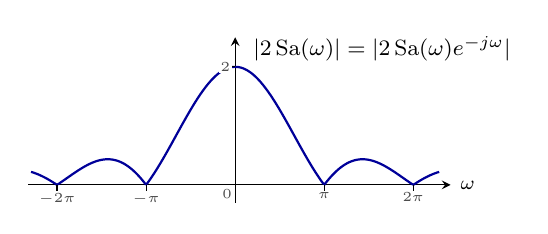
\begin{tikzpicture}[x=0.36cm,y=0.75cm]
  \taxes[\omega]{-7.3}{7.6}{2.5}{-0.3}
  \draw[sig,domain=-7.2:7.2,samples=240] plot (\x,{abs(2*sin(\x r)/\x)});
  \foreach \p/\l in {-6.2832/-2\pi,-3.1416/-\pi,3.1416/\pi,6.2832/2\pi}{\xt{\p}{\l}}
  \yt{2}{2}
  \node[font=\footnotesize,anchor=west] at (0.3,2.3) {$|2\Sa(\omega)|=|2\Sa(\omega)e^{-j\omega}|$};
\end{tikzpicture}
\caption{左：$0\sim2$ 上的方波是 $-1\sim1$ 上的方波右移 $1$。右：两者的幅度谱相同，平移只改变相位。}
\label{fig:tshift}
\end{figure}

\example{$0\sim2$ 上的方波}{$2\Sa(\omega)e^{-j\omega}$}{}
\point{分解动作。}设 $y(t)$ 是 $-1\sim1$ 上高 $1$ 的方波，$y(t)\xrightarrow{\F}2\Sa(\omega)$。$x(t)=y(t-1)$ 是它右移 $1$，由时移性质
\[
x(t)\xrightarrow{\F}2\Sa(\omega)\,e^{-j\omega}.
\]
\point{连续动作。}分解动作做多了，可以一步写出：先写 $\Sa$，方波移到中间后半宽是 $1$，写 $\Sa(\omega)$；乘面积 $2$；向右移了 $1$，再乘 $e^{-j\omega}$。

\example{两个分开的方波（用时移性质）}{$4\Sa(\omega)\cos(3\omega)$}{}
仍是 $-4\sim-2$ 和 $2\sim4$ 上为 $1$ 的信号，这次同时用时移性质和线性性质。设 $y(t)$ 是 $-1\sim1$ 上高 $1$ 的方波：
\begin{itemize}[nosep]
\item 右边的方波是 $y(t-3)$，$t_0=3$：$\F[y(t-3)]=\F[y(t)]\,e^{-j3\omega}=2\Sa(\omega)e^{-j3\omega}$；
\item 左边的方波是 $y(t+3)$（加号左移，减号右移），$t-(-3)=t+3$，所以 $t_0=-3$：$\F[y(t+3)]=2\Sa(\omega)e^{j3\omega}$；
\item 由线性性质相加：
\[
X(j\omega)=2\Sa(\omega)\big[e^{-j3\omega}+e^{j3\omega}\big]=2\Sa(\omega)\cdot2\cos(3\omega)=4\Sa(\omega)\cos(3\omega).
\]
\end{itemize}
最后一步用了常用公式 $e^{j\alpha}+e^{-j\alpha}=2\cos\alpha$。写到 $2\Sa(\omega)[e^{-j3\omega}+e^{j3\omega}]$ 不算错，但还能化简。

\begin{remember}
\textbf{关于纵轴对称复制。}把同一个波形 $x(t)$ 分别右移、左移 $t_0$ 再相加，得到关于纵轴对称的两份，它的傅里叶变换是
\[
x(t-t_0)+x(t+t_0)\xrightarrow{\F}2X(j\omega)\cos(\omega t_0).
\]
原因：右边那份多出 $e^{-j\omega t_0}$，左边那份多出 $e^{j\omega t_0}$，加起来是 $2\cos(\omega t_0)$。做题时把波形移到中间写出变换，再乘 $2\cos(\omega t_0)$。
\end{remember}

\begin{figure}[H]
\centering
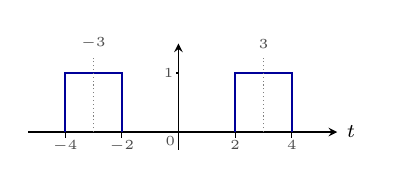
\begin{tikzpicture}[x=0.36cm,y=0.75cm]
  \taxes{-5.3}{5.6}{1.5}{-0.3}
  \rectp{-4}{-2}{1}\rectp{2}{4}{1}
  \foreach \p in {-4,-2,2,4}{\xt{\p}{\p}}\yt{1}{1}
  \draw[gray,densely dotted] (-3,0) -- (-3,1.25); \draw[gray,densely dotted] (3,0) -- (3,1.25);
  \node[font=\tiny,gray!60!black,anchor=south] at (-3,1.25) {$-3$};
  \node[font=\tiny,gray!60!black,anchor=south] at (3,1.25) {$3$};
\end{tikzpicture}
\hspace{5mm}
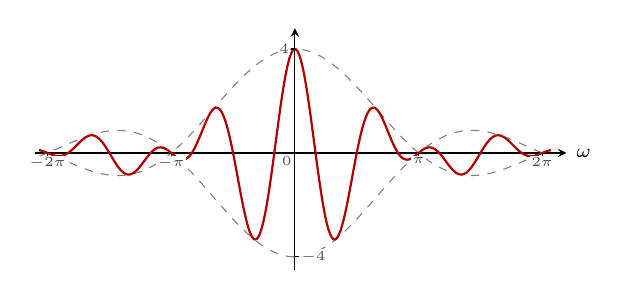
\begin{tikzpicture}[x=0.5cm,y=0.33cm]
  \taxes[\omega]{-6.6}{6.9}{4.8}{-4.5}
  \draw[gray,dashed,domain=-6.5:6.5,samples=200] plot (\x,{4*sin(\x r)/\x});
  \draw[gray,dashed,domain=-6.5:6.5,samples=200] plot (\x,{-4*sin(\x r)/\x});
  \draw[res,domain=-6.5:6.5,samples=300] plot (\x,{4*sin(\x r)*cos(3*\x r)/\x});
  \foreach \p/\l in {-6.2832/-2\pi,-3.1416/-\pi,3.1416/\pi,6.2832/2\pi}{\xt{\p}{\l}}
  \yt{4}{4}\ytr{-4}{-4}
\end{tikzpicture}
\caption{左：关于纵轴对称的两个方波，中心在 $\pm3$。右：它的傅里叶变换 $4\Sa(\omega)\cos(3\omega)$（红），在包络 $\pm4\Sa(\omega)$（灰虚线）之间振荡。}
\label{fig:sym}
\end{figure}

\example{两个阶跃}{$u(t-1)$ 与 $u(-1-t)$}{}
求 $u(t-1)$ 和 $u(-1-t)$ 的傅里叶变换（图~\ref{fig:steps}）。
\begin{figure}[H]
\centering
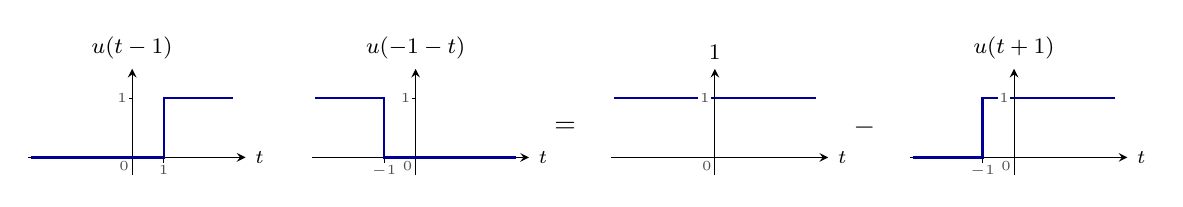
\begin{tikzpicture}[x=0.4cm,y=0.75cm]
  \begin{scope}
    \taxes{-3.3}{3.6}{1.5}{-0.3}
    \draw[sig] (-3.2,0) -- (1,0) -- (1,1) -- (3.2,1);
    \xt{1}{1}\yt{1}{1}
    \node[font=\footnotesize,anchor=south] at (0,1.5) {$u(t-1)$};
  \end{scope}
  \begin{scope}[xshift=3.6cm]
    \taxes{-3.3}{3.6}{1.5}{-0.3}
    \draw[sig] (-3.2,1) -- (-1,1) -- (-1,0) -- (3.2,0);
    \xt{-1}{-1}\yt{1}{1}
    \node[font=\footnotesize,anchor=south] at (0,1.5) {$u(-1-t)$};
  \end{scope}
  \node at (13.75,0.5) {$=$};
  \begin{scope}[xshift=7.4cm]
    \taxes{-3.3}{3.6}{1.5}{-0.3}
    \draw[sig] (-3.2,1) -- (3.2,1);
    \yt{1}{1}
    \node[font=\footnotesize,anchor=south] at (0,1.5) {$1$};
  \end{scope}
  \node at (23.25,0.5) {$-$};
  \begin{scope}[xshift=11.2cm]
    \taxes{-3.3}{3.6}{1.5}{-0.3}
    \draw[sig] (-3.2,0) -- (-1,0) -- (-1,1) -- (3.2,1);
    \xt{-1}{-1}\yt{1}{1}
    \node[font=\footnotesize,anchor=south] at (0,1.5) {$u(t+1)$};
  \end{scope}
\end{tikzpicture}
\caption{$u(t-1)$ 是 $u(t)$ 右移 $1$；$u(-1-t)$ 等于常数 $1$ 减去 $u(t)$ 左移 $1$。}
\label{fig:steps}
\end{figure}

\point{$u(t-1)$。}$u(t)$ 右移一个单位，乘 $e^{-j\omega}$：
\[
\F[u(t-1)]=\Big[\frac1{j\omega}+\pi\delta(\omega)\Big]e^{-j\omega}=\frac{e^{-j\omega}}{j\omega}+\pi e^{-j\omega}\delta(\omega).
\]
写成 $\pi e^{-j\omega}\delta(\omega)$ 不算错，但还能化简一步：用冲激函数的性质 $x(\omega)\delta(\omega)=x(0)\delta(\omega)$，$e^{-j0}=1$，所以
\[
\F[u(t-1)]=\frac{e^{-j\omega}}{j\omega}+\pi\delta(\omega).
\]
\point{$u(-1-t)$。}稍复杂一点。$u(-1-t)=u(-(t+1))$ 在 $t<-1$ 时为 $1$，它等于 $1-u(t+1)$；$u(t+1)$ 是 $u(t)$ 左移一个单位，乘 $e^{j\omega}$：
\[
\begin{aligned}
\F[u(-1-t)]&=2\pi\delta(\omega)-\Big[\frac1{j\omega}+\pi\delta(\omega)\Big]e^{j\omega}\\
&=2\pi\delta(\omega)-\frac{e^{j\omega}}{j\omega}-\pi\delta(\omega)\\
&=\pi\delta(\omega)-\frac{e^{j\omega}}{j\omega}.
\end{aligned}
\]
中间一步同样用了 $\pi e^{j\omega}\delta(\omega)=\pi\delta(\omega)$。

\point{易错点。}方括号前的负号要乘到括号里的每一项上：$\pi\delta(\omega)$ 前面是减号。漏乘会得到 $3\pi\delta(\omega)-\frac{e^{j\omega}}{j\omega}$ 这样的错误结果。验算：$u(-t)$ 是 $u(t)$ 的翻转，$u(-t)\xrightarrow{\F}-\frac1{j\omega}+\pi\delta(\omega)$；$u(-1-t)$ 是 $u(-t)$ 左移 $1$，乘 $e^{j\omega}$ 得 $-\frac{e^{j\omega}}{j\omega}+\pi\delta(\omega)$，与上面一致。

\example{线性相位}{$x(t)=\dfrac{\sin[2(t-2)]}{\pi(t-2)}$}{}
已知 $X(j\omega)=|X(j\omega)|\,e^{j\theta(\omega)}$，其中 $|X(j\omega)|$ 是 $-2\sim2$ 上高 $1$ 的方波，$\theta(\omega)=-2\omega$（图~\ref{fig:linphase}）。求反变换 $x(t)$。这是时移性质里相对难的题。

\point{先只看幅度。}如果只有 $|X(j\omega)|$ 这个方波，由公式 \cn5（$\omega_c=2$），它对应 $\dfrac{\sin(2t)}{\pi t}$。

\point{再乘相位因子。}$e^{j\theta(\omega)}=e^{-j2\omega}=e^{-j\omega\cdot2}$。时移性质说 $e^{-j\omega t_0}$ 对应时域延时 $t_0$，这里 $t_0=2$。把 $\dfrac{\sin(2t)}{\pi t}$ 中所有的 $t$ 换成 $t-2$：
\[
x(t)=\frac{\sin[2(t-2)]}{\pi(t-2)} .
\]

\begin{remember}
\textbf{频域的线性相位对应时域的延时。}相位是 $\omega$ 的线性函数 $\theta(\omega)=-\omega t_0$ 时，时域延时 $t_0$；延时多少由线性相位的斜率决定（斜率为 $-t_0$）。这个概念后面还会用到。
\end{remember}

\begin{figure}[H]
\centering
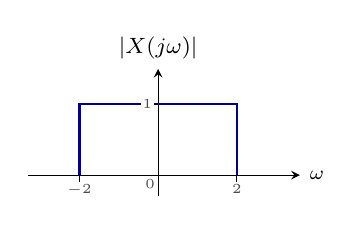
\begin{tikzpicture}[x=0.5cm,y=0.9cm]
  \taxes[\omega]{-3.3}{3.6}{1.5}{-0.3}
  \rectp{-2}{2}{1}
  \xt{-2}{-2}\xt{2}{2}\yt{1}{1}
  \node[font=\footnotesize,anchor=south] at (0,1.5) {$|X(j\omega)|$};
\end{tikzpicture}
\hspace{3mm}
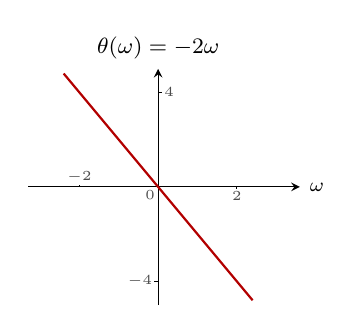
\begin{tikzpicture}[x=0.5cm,y=0.3cm]
  \taxes[\omega]{-3.3}{3.6}{5}{-5}
  \draw[res] (-2.4,4.8) -- (2.4,-4.8);
  \xtu{-2}{-2}\xt{2}{2}\ytr{4}{4}\yt{-4}{-4}
  \node[font=\footnotesize,anchor=south] at (0,5) {$\theta(\omega)=-2\omega$};
\end{tikzpicture}
\hspace{3mm}
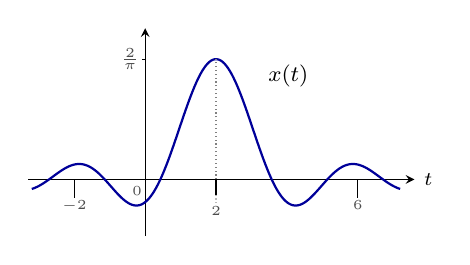
\begin{tikzpicture}[x=0.45cm,y=2.4cm]
  \taxes{-3.3}{7.6}{0.8}{-0.3}
  \draw[sig,domain=-3.2:7.2,samples=200] plot (\x,{sin(2*(\x-2) r)/(pi*(\x-2))});
  \draw[gray,densely dotted] (2,0) -- (2,0.6366);
  \xtl{2}{2}{-0.13}\xt{-2}{-2}\xt{6}{6}
  \yt{0.6366}{\frac2\pi}
  \node[font=\footnotesize,anchor=west] at (3.2,0.55) {$x(t)$};
\end{tikzpicture}
\caption{幅度谱是方波、相位谱是斜率为 $-2$ 的直线：时域是 $\frac{\sin(2t)}{\pi t}$ 延时 $2$，峰值 $\frac2\pi$ 从 $t=0$ 移到 $t=2$。}
\label{fig:linphase}
\end{figure}

%==================================================================
\section{频移性质}\label{sec:fshift}
\begin{remember}
\textbf{\cn3 频移性质（教材 3.4.3）。}若 $x(t)\xrightarrow{\F}X(j\omega)$，则
\[
x(t)\,e^{j\omega_0t}\xrightarrow{\F}X\big(j(\omega-\omega_0)\big).
\]
\end{remember}

\point{证明。}
\[
X(j\omega)=\int_{-\infty}^{+\infty}x(t)\,e^{-j\omega t}\,\dd t ,
\]
\[
\begin{aligned}
\F\big[x(t)e^{j\omega_0t}\big]&=\int_{-\infty}^{+\infty}x(t)\,e^{j\omega_0t}\,e^{-j\omega t}\,\dd t\\
&=\int_{-\infty}^{+\infty}x(t)\,e^{-j(\omega-\omega_0)t}\,\dd t\\
&=X\big(j(\omega-\omega_0)\big).
\end{aligned}
\]
最后一步对照 $X(j\omega)$ 的定义式：定义式里 $e$ 的指数是 $-j\omega t$、左边是 $X(j\omega)$；这里指数里的 $\omega$ 换成了 $\omega-\omega_0$，左边也就把 $\omega$ 换成 $\omega-\omega_0$。

\subsection{推出公式 \texorpdfstring{\cn7}{⑦}：余弦与正弦}\label{sub:cossin}
公式 \cn7 要记住，而它是由频移性质推出来的。要用到
\[
\cos(\omega_0t)=\frac12\big(e^{j\omega_0t}+e^{-j\omega_0t}\big),\qquad
\sin(\omega_0t)=\frac1{2j}\big(e^{j\omega_0t}-e^{-j\omega_0t}\big),
\]
以及第三块积木 $1\xrightarrow{\F}2\pi\delta(\omega)$。

\point{余弦。}$1\cdot e^{j\omega_0t}$ 是 $x(t)=1$ 乘 $e^{j\omega_0t}$，由频移性质
\[
e^{j\omega_0t}\xrightarrow{\F}2\pi\delta(\omega-\omega_0),\qquad e^{-j\omega_0t}\xrightarrow{\F}2\pi\delta(\omega+\omega_0).
\]
乘上 $\frac12$，$2\pi$ 里的 $2$ 被约掉，再相加：
\[
\cos(\omega_0t)\xrightarrow{\F}\pi\big[\delta(\omega+\omega_0)+\delta(\omega-\omega_0)\big].
\]
\point{正弦。}步骤完全一样，唯一不同是系数 $\frac1{2j}$ 和中间的减号：
\[
\sin(\omega_0t)\xrightarrow{\F}\frac\pi j\big[\delta(\omega-\omega_0)-\delta(\omega+\omega_0)\big].
\]

\begin{figure}[H]
\centering
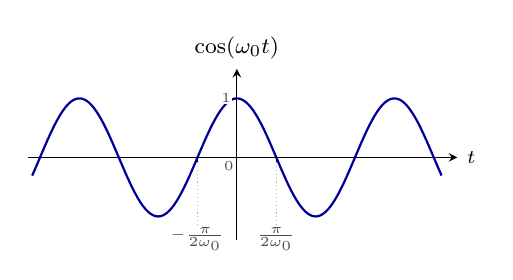
\begin{tikzpicture}[x=0.5cm,y=0.75cm]
  \taxes{-5.3}{5.6}{1.5}{-1.4}
  \draw[sig,domain=-5.2:5.2,samples=160] plot (\x,{cos(90*\x)});
  \xtl{1}{\frac{\pi}{2\omega_0}}{-1.15}\xtl{-1}{-\frac{\pi}{2\omega_0}}{-1.15}
  \yt{1}{1}
  \node[font=\footnotesize,anchor=south] at (0,1.5) {$\cos(\omega_0t)$};
\end{tikzpicture}
\hspace{4mm}
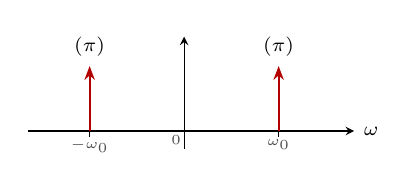
\begin{tikzpicture}[x=0.6cm,y=0.75cm]
  \taxes[\omega]{-3.3}{3.6}{1.6}{-0.3}
  \draw[imp,res] (-2,0) -- (-2,1.1); \draw[imp,res] (2,0) -- (2,1.1);
  \node[font=\scriptsize,anchor=south] at (-2,1.1) {$(\pi)$};
  \node[font=\scriptsize,anchor=south] at (2,1.1) {$(\pi)$};
  \xt{-2}{-\omega_0}\xt{2}{\omega_0}
\end{tikzpicture}

\vspace{2mm}
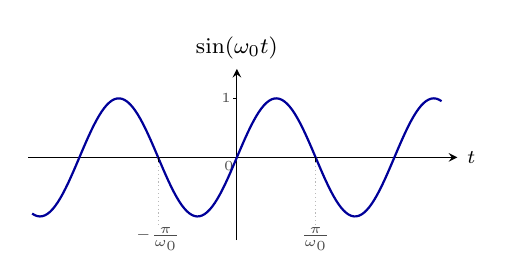
\begin{tikzpicture}[x=0.5cm,y=0.75cm]
  \taxes{-5.3}{5.6}{1.5}{-1.4}
  \draw[sig,domain=-5.2:5.2,samples=160] plot (\x,{sin(90*\x)});
  \xtl{2}{\frac{\pi}{\omega_0}}{-1.15}\xtl{-2}{-\frac{\pi}{\omega_0}}{-1.15}
  \yt{1}{1}
  \node[font=\footnotesize,anchor=south] at (0,1.5) {$\sin(\omega_0t)$};
\end{tikzpicture}
\hspace{4mm}
\begin{tikzpicture}[x=0.6cm,y=0.75cm]
  \taxes[\omega]{-3.3}{3.6}{1.6}{-1.5}
  \draw[imp,res] (2,0) -- (2,1.1); \draw[imp,res] (-2,0) -- (-2,-1.1);
  \node[font=\scriptsize,anchor=south] at (2,1.1) {$(\frac\pi j)$};
  \node[font=\scriptsize,anchor=north] at (-2,-1.1) {$(-\frac\pi j)$};
  \xtu{-2}{-\omega_0}\xt{2}{\omega_0}
\end{tikzpicture}
\caption{上：$\cos(\omega_0t)$ 的过零点在 $\pm\frac{\pi}{2\omega_0}$，频谱是 $\pm\omega_0$ 处两个强度为 $\pi$ 的冲激。下：$\sin(\omega_0t)$ 的过零点在 $0,\pm\frac{\pi}{\omega_0}$，频谱在 $\omega_0$ 处强度为 $\frac\pi j$（朝上画）、在 $-\omega_0$ 处为 $-\frac\pi j$（朝下画）。}
\label{fig:cossin}
\end{figure}

\begin{remember}
余弦、正弦的傅里叶变换，式子和图都要记住（图~\ref{fig:cossin}）。正弦的两个冲激哪个朝上、哪个朝下容易记混，要特别留意。
\end{remember}

\point{正弦的另一种写法。}有些书写成
\[
\sin(\omega_0t)\xrightarrow{\F}j\pi\big[\delta(\omega+\omega_0)-\delta(\omega-\omega_0)\big],
\]
图上 $-\omega_0$ 处为 $j\pi$、$\omega_0$ 处为 $-j\pi$。两种写法是一样的：$\frac1j=-j$，把 $j$ 从分母拿到分子，多出一个负号，括号里两项的顺序正好颠倒。本篇按 $\frac\pi j$ 的写法，另一种写法同样正确。

\subsection{乘以余弦、正弦}\label{sub:modu}
\begin{remember}
若 $x(t)\xrightarrow{\F}X(j\omega)$，则（教材第 105 页式 3-76、3-77）
\[
\begin{aligned}
x(t)\cos(\omega_0t)&\xrightarrow{\F}\frac12\Big[X\big(j(\omega-\omega_0)\big)+X\big(j(\omega+\omega_0)\big)\Big],\\
x(t)\sin(\omega_0t)&\xrightarrow{\F}\frac1{2j}\Big[X\big(j(\omega-\omega_0)\big)-X\big(j(\omega+\omega_0)\big)\Big].
\end{aligned}
\]
\end{remember}
\point{推导。}把余弦拆开：
\[
x(t)\cos(\omega_0t)=\frac12x(t)e^{j\omega_0t}+\frac12x(t)e^{-j\omega_0t},
\]
两项分别用频移性质，马上得到第一式；正弦同理。教材上正弦一式写成
\[
\frac j2\Big[X\big(j(\omega+\omega_0)\big)-X\big(j(\omega-\omega_0)\big)\Big],
\]
理由与上面一样：$j$ 放在分母还是分子，括号里两项的顺序要相应交换，两种写法都对。

后面讲完调制性质，这两个结论会变得更直观，那时再回到这里。

\begin{figure}[H]
\centering
\begin{tikzpicture}[x=0.5cm,y=1.0cm]
  \taxes[\omega]{-5.3}{5.6}{1.4}{-0.3}
  \trip{-1}{0}{1}{1}
  \xt{-1}{-1}\xt{1}{1}\yt{1}{1}
  \node[font=\footnotesize,anchor=south] at (0,1.4) {$X(j\omega)$};
\end{tikzpicture}
\hspace{6mm}
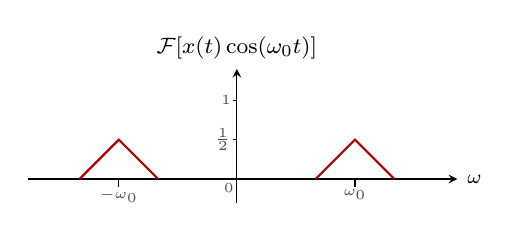
\begin{tikzpicture}[x=0.5cm,y=1.0cm]
  \taxes[\omega]{-5.3}{5.6}{1.4}{-0.3}
  \trip[res]{-4}{-3}{-2}{0.5}\trip[res]{2}{3}{4}{0.5}
  \xt{-3}{-\omega_0}\xt{3}{\omega_0}\yt{0.5}{\frac12}\yt{1}{1}
  \node[font=\footnotesize,anchor=south] at (0,1.4) {$\F[x(t)\cos(\omega_0t)]$};
\end{tikzpicture}
\caption{乘以 $\cos(\omega_0t)$：原来的频谱（左）搬到 $\pm\omega_0$ 两处，高度各减半（右）。}
\label{fig:modu}
\end{figure}

\point{跳过的内容。}教材 3.4.4「共轭与共轭对称性」不是不重要，后面专门用一节课讲；3.4.6、3.4.7 也放到后面。

%==================================================================
\section{微分性质}\label{sec:diff}
微分性质严格说分两种：时域微分和频域微分。

\subsection{时域微分}\label{sub:tdiff}
\begin{remember}
\textbf{\cn4 时域微分性质（教材 3.4.5，第 106 页）。}若 $x(t)\xrightarrow{\F}X(j\omega)$，则
\[
\frac{\dd x(t)}{\dd t}\xrightarrow{\F}j\omega\,X(j\omega).
\]
\end{remember}

\point{证明。}反过来证更好证，用反变换公式：
\[
x(t)=\frac1{2\pi}\int_{-\infty}^{+\infty}X(j\omega)\,e^{j\omega t}\,\dd\omega .
\]
两边对 $t$ 求导。右边只有 $e^{j\omega t}$ 含 $t$，其他地方都是 $\omega$：
\[
\frac{\dd x(t)}{\dd t}=\frac1{2\pi}\int_{-\infty}^{+\infty}X(j\omega)\Big[\frac{\dd(e^{j\omega t})}{\dd t}\Big]\dd\omega
=\frac1{2\pi}\int_{-\infty}^{+\infty}\big[j\omega X(j\omega)\big]\,e^{j\omega t}\,\dd\omega .
\]
求导把 $j\omega$ 拿了出来，和前面的 $X(j\omega)$ 合在一起。按反变换的定义，右边正是 $j\omega X(j\omega)$ 的反变换，所以 $\frac{\dd x(t)}{\dd t}$ 与 $j\omega X(j\omega)$ 是一对傅里叶变换。

\example{冲激函数的各阶导数}{$\delta^{(n)}(t)\xrightarrow{\F}(j\omega)^n$}{}
$\delta(t)\xrightarrow{\F}1$，所以
\[
\delta'(t)=\frac{\dd\delta(t)}{\dd t}\xrightarrow{\F}j\omega\cdot1=j\omega,\qquad
\delta''(t)\xrightarrow{\F}(j\omega)^2,\qquad
\delta^{(n)}(t)=\frac{\dd^n\delta(t)}{\dd t^n}\xrightarrow{\F}(j\omega)^n .
\]

\subsection{频域微分}\label{sub:fdiff}
\begin{remember}
\textbf{\cn5 频域微分性质（教材第 114 页表 3-1 第 11 条）。}若 $x(t)\xrightarrow{\F}X(j\omega)$，则
\[
t\,x(t)\xrightarrow{\F}j\,\frac{\dd X(j\omega)}{\dd\omega}.
\]
\end{remember}

\point{证明。}
\[
X(j\omega)=\int_{-\infty}^{+\infty}x(t)\,e^{-j\omega t}\,\dd t .
\]
两边对 $\omega$ 求导。右边只有 $e^{-j\omega t}$ 含 $\omega$：
\[
\frac{\dd X(j\omega)}{\dd\omega}=\int_{-\infty}^{+\infty}x(t)\Big[\frac{\dd(e^{-j\omega t})}{\dd\omega}\Big]\dd t
=\int_{-\infty}^{+\infty}\big[-jt\,x(t)\big]\,e^{-j\omega t}\,\dd t .
\]
按傅里叶变换的定义，$-jt\,x(t)$ 与 $\frac{\dd X(j\omega)}{\dd\omega}$ 是一对傅里叶变换：
\[
-jt\,x(t)\xrightarrow{\F}\frac{\dd X(j\omega)}{\dd\omega}.
\]
用线性性质两边同乘 $j$，$j\cdot(-j)=1$，得 $t\,x(t)\xrightarrow{\F}j\,\frac{\dd X(j\omega)}{\dd\omega}$。

\example{$t\,e^{-at}u(t)$}{$\dfrac1{(a+j\omega)^2}$}{}
这个性质有一个很常见的运用。由公式 \cn1，$e^{-at}u(t)\xrightarrow{\F}\frac1{a+j\omega}$（$a>0$），所以
\[
t\,e^{-at}u(t)\xrightarrow{\F}j\,\frac{\dd\,(a+j\omega)^{-1}}{\dd\omega}.
\]
求导时负号拿下来，指数变成 $-2$，别忘了还要对 $a+j\omega$ 求导，再乘一个 $j$：
\[
j\cdot(-1)(a+j\omega)^{-2}\cdot j=\frac1{(a+j\omega)^2}
\]
（两个 $j$ 相乘得 $-1$，与前面的 $-1$ 抵消）。这就是教材第 116 页续表最下面一行。

\point{再推一次。}
\[
t^2e^{-at}u(t)\xrightarrow{\F}j\,\frac{\dd\,(a+j\omega)^{-2}}{\dd\omega}=j\cdot(-2)(a+j\omega)^{-3}\cdot j=\frac2{(a+j\omega)^3}.
\]
\point{通用公式。}$n=1$ 时分母是 $(a+j\omega)^2$、分子是 $1$；$n=2$ 时分母是 $(a+j\omega)^3$、分子是 $2$；再推一次分子是 $3!$。所以
\[
t^n e^{-at}u(t)\xrightarrow{\F}\frac{n!}{(a+j\omega)^{n+1}},
\]
与教材的结果一致，可以用数学归纳法证明。这个公式不必背：$n>1$ 的情况很少用到，真碰到了，知道上面两个性质也能推出来，只是花的时间稍长。

\begin{figure}[H]
\centering
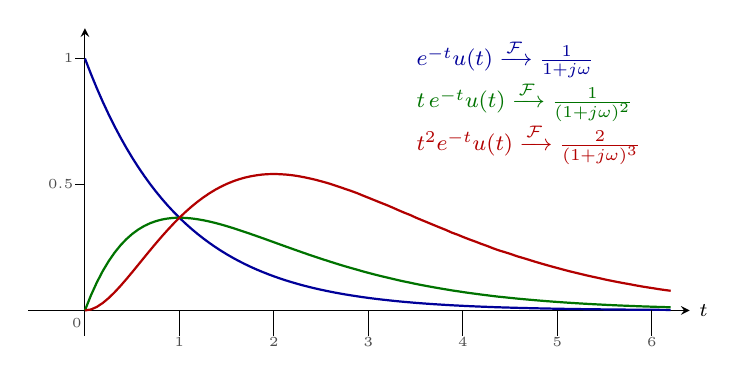
\begin{tikzpicture}[x=1.2cm,y=3.2cm]
  \taxes{-0.6}{6.4}{1.12}{-0.1}
  \draw[sig,domain=0:6.2,samples=100] plot (\x,{exp(-\x)});
  \draw[grn,domain=0:6.2,samples=100] plot (\x,{\x*exp(-\x)});
  \draw[res,domain=0:6.2,samples=100] plot (\x,{\x*\x*exp(-\x)});
  \foreach \p in {1,2,3,4,5,6}{\xt{\p}{\p}}
  \yt{1}{1}\yt{0.5}{0.5}
  \node[sig,font=\footnotesize,anchor=west] at (3.4,1.0) {$e^{-t}u(t)\xrightarrow{\F}\frac1{1+j\omega}$};
  \node[grn,font=\footnotesize,anchor=west] at (3.4,0.83) {$t\,e^{-t}u(t)\xrightarrow{\F}\frac1{(1+j\omega)^2}$};
  \node[res,font=\footnotesize,anchor=west] at (3.4,0.66) {$t^2e^{-t}u(t)\xrightarrow{\F}\frac2{(1+j\omega)^3}$};
\end{tikzpicture}
\caption{$a=1$ 时的单边指数信号及它乘 $t$、乘 $t^2$ 的结果。时域每多乘一个 $t$，频域就对 $\omega$ 求一次导再乘 $j$。}
\label{fig:fdiff}
\end{figure}

%==================================================================
\section{时域卷积性质}\label{sec:conv}
\begin{remember}
\textbf{\cn6 时域卷积性质（教材 3.4.9，第 112 页；非常重要）。}若 $x(t)\xrightarrow{\F}X(j\omega)$，$h(t)\xrightarrow{\F}H(j\omega)$，则
\[
x(t)*h(t)\xrightarrow{\F}X(j\omega)\,H(j\omega).
\]
\textbf{时域卷积等于频域相乘}：时域上两个信号卷积得到的新信号，它的傅里叶变换等于两个信号傅里叶变换的乘积。
\end{remember}

\point{证明。}第一步要把第二章的知识连起来。设
\[
y(t)=x(t)*h(t)=\int_{-\infty}^{+\infty}x(\tau)\,h(t-\tau)\,\dd\tau .
\]
按定义，并把 $y(t)$ 直接代进去：
\[
\begin{aligned}
Y(j\omega)&=\int_{-\infty}^{+\infty}y(t)\,e^{-j\omega t}\,\dd t
=\int_{-\infty}^{+\infty}\Big[\int_{-\infty}^{+\infty}x(\tau)\,h(t-\tau)\,\dd\tau\Big]e^{-j\omega t}\,\dd t\\
&=\Big[\int_{-\infty}^{+\infty}x(\tau)\,e^{-j\omega\tau}\,\dd\tau\Big]\Big[\int_{-\infty}^{+\infty}h(t-\tau)\,e^{-j\omega(t-\tau)}\,\dd t\Big].
\end{aligned}
\]
核心在这一步：改变积分次序，同时把 $e^{-j\omega t}$ 拆成 $e^{-j\omega\tau}$ 和 $e^{-j\omega(t-\tau)}$，两者相乘正好是 $e^{-j\omega t}$。

\point{更严格的写法：换元。}设
\[
t'=t-\tau,\qquad \tau'=\tau .
\]
雅可比行列式(Jacobian determinant)为
\[
\begin{vmatrix}\dfrac{\partial t'}{\partial t}&\dfrac{\partial t'}{\partial\tau}\\[2ex]\dfrac{\partial\tau'}{\partial t}&\dfrac{\partial\tau'}{\partial\tau}\end{vmatrix}
=\begin{vmatrix}1&-1\\0&1\end{vmatrix}=1 .
\]
行列式等于 $1$，换元后面积元前面乘的就是 $1$。$t-\tau$ 全部换成 $t'$：
\[
Y(j\omega)=\Big[\int_{-\infty}^{+\infty}x(\tau')\,e^{-j\omega\tau'}\,\dd\tau'\Big]\Big[\int_{-\infty}^{+\infty}h(t')\,e^{-j\omega t'}\,\dd t'\Big]=X(j\omega)\,H(j\omega).
\]
按傅里叶变换的定义，第一个括号是 $X(j\omega)$，第二个括号是 $H(j\omega)$。

有了卷积性质，搭积木的方法丰富了很多，可以写出更多没见过的信号的傅里叶变换。下面先做题，第 \ref{sec:lti} 节再用它回答第三章开头的问题。

\subsection{三角波：两个方波的卷积}\label{sub:tri}
\begin{figure}[H]
\centering
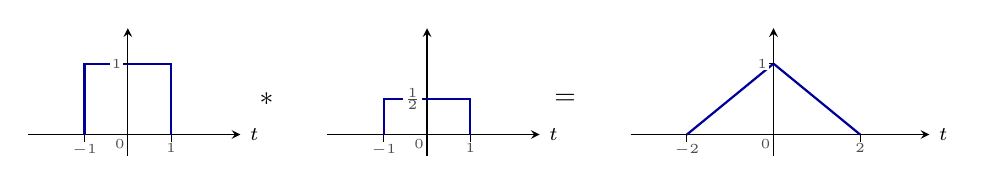
\begin{tikzpicture}[x=0.55cm,y=0.9cm]
  \begin{scope}
    \taxes{-2.3}{2.6}{1.5}{-0.3}
    \rectp{-1}{1}{1}
    \xt{-1}{-1}\xt{1}{1}\yt{1}{1}
  \end{scope}
  \node at (3.2,0.5) {$*$};
  \begin{scope}[xshift=3.8cm]
    \taxes{-2.3}{2.6}{1.5}{-0.3}
    \rectp{-1}{1}{0.5}
    \xt{-1}{-1}\xt{1}{1}\yt{0.5}{\frac12}
  \end{scope}
  \node at (10.1,0.5) {$=$};
  \begin{scope}[xshift=8.2cm]
    \taxes{-3.3}{3.6}{1.5}{-0.3}
    \trip{-2}{0}{2}{1}
    \xt{-2}{-2}\xt{2}{2}\yt{1}{1}
  \end{scope}
\end{tikzpicture}

\vspace{2mm}
\begin{tikzpicture}[x=0.5cm,y=0.95cm]
  \taxes[\omega]{-7.3}{7.6}{2.4}{-0.6}
  \draw[sig,dashed,domain=-7.2:7.2,samples=240] plot (\x,{2*sin(\x r)/\x});
  \draw[grn,dotted,domain=-7.2:7.2,samples=240] plot (\x,{sin(\x r)/\x});
  \draw[res,domain=-7.2:7.2,samples=240] plot (\x,{2*(sin(\x r)/\x)^2});
  \foreach \p/\l in {-6.2832/-2\pi,-3.1416/-\pi,3.1416/\pi,6.2832/2\pi}{\xt{\p}{\l}}
  \yt{1}{1}\yt{2}{2}
  \node[res,font=\footnotesize,anchor=west] at (0.3,2.15) {$2\Sa^2(\omega)$};
  \node[sig,font=\footnotesize,anchor=west] at (3.5,1.2) {虚线 $2\Sa(\omega)$};
  \node[grn,font=\footnotesize,anchor=west] at (3.5,0.8) {点线 $\Sa(\omega)$};
\end{tikzpicture}
\caption{上：$-2\sim2$、高 $1$ 的三角波等于两个 $-1\sim1$ 方波（高 $1$ 和 $\frac12$）的卷积。下：频域里两个 Sa 相乘得到 $2\Sa^2(\omega)$，处处非负。}
\label{fig:tri}
\end{figure}

\example{三角波}{$2\Sa^2(\omega)$}{}
$x(t)$ 是 $-2\sim2$ 上、顶点高 $1$ 的三角波。三角波是两个长度一致的方波的卷积；方波的傅里叶变换已经知道，时域卷积等于频域相乘，把两个方波的变换乘起来就得到三角波的变换。

\point{分解动作。}三角波 $=$ $-1\sim1$ 上高 $E_1$ 的方波 $*$ $-1\sim1$ 上高 $E_2$ 的方波。两个方波各贡献一个 $\Sa(\omega)$，乘起来是 $\Sa^2(\omega)$。难点在于两个方波的幅度怎么定：卷积后顶点的高度是「重叠长度 $2$ $\times E_1E_2$」，要等于 $1$，所以
\[
2E_1E_2=1 .
\]
满足这个条件的取法不止一种，只要乘积对就行。比如 $E_1=1$、$E_2=\frac12$：
\[
X(j\omega)=\underbrace{2\Sa(\omega)}_{E_1=1}\cdot\underbrace{\Sa(\omega)}_{E_2=\frac12}=2\Sa^2(\omega).
\]
\point{连续动作。}不用凑 $E_1$、$E_2$：两个方波贡献 $\Sa^2(\omega)$（括号里是方波的半宽 $1$），前面的系数直接写三角形的面积 $\frac{4\times1}2=2$。

\begin{remember}
\textbf{系数就是面积。}设 $X(j\omega)=A\Sa^2(\omega)$。由定义，$\omega=0$ 时
\[
X(j0)=\int_{-\infty}^{+\infty}x(t)\,e^{-j0t}\,\dd t=\int_{-\infty}^{+\infty}x(t)\,\dd t ;
\]
另一方面 $X(j0)=A\Sa^2(0)=A$。所以 $A=\int_{-\infty}^{+\infty}x(t)\,\dd t$，正好是三角形的面积。

\textbf{三角波的快速写法：}脑子里过一下「两个方波卷积」，写出 $\Sa^2(\text{方波半宽}\times\omega)$，再把三角波的面积写在前面。方波的半宽是三角波底宽的四分之一。
\end{remember}

\example{顶点高 2 的三角波}{$8\Sa^2(2\omega)$}{}
$x(t)$ 是 $-4\sim4$ 上、顶点高 $2$ 的三角波。它由两个 $-2\sim2$ 的方波卷积而成，写 $\Sa^2(2\omega)$；面积 $\frac{8\times2}{2}=8$：
\[
X(j\omega)=8\Sa^2(2\omega).
\]

\example{一般的三角脉冲}{$\dfrac{E\tau}2\Sa^2\Big(\dfrac\tau4\omega\Big)$}{教材第 107 页例 3-6}
$x(t)$ 是 $-\frac\tau2\sim\frac\tau2$ 上、顶点高 $E$ 的三角波。方波半宽是 $\frac\tau4$，写 $\Sa^2(\frac\tau4\omega)$；面积是 $\frac{\tau E}{2}$：
\[
X(j\omega)=\frac{E\tau}2\Sa^2\Big(\frac\tau4\omega\Big),
\]
与教材第 108 页式 3-85 的结果完全一样。教材用的方法要复杂得多。

\subsection{梯形：两个不等宽方波的卷积}\label{sub:trap}
\begin{remember}
$-a\sim a$ 上高 $E_1$ 的方波，卷积 $-b\sim b$ 上高 $E_2$ 的方波（$a>b$），得到一个梯形：四个转折点是
\[
-a-b,\qquad b-a,\qquad a-b,\qquad a+b ,
\]
顶部高度是 $2bE_1E_2$（图~\ref{fig:trap}）。核心是记住底下这四个坐标。
\end{remember}

\begin{figure}[H]
\centering
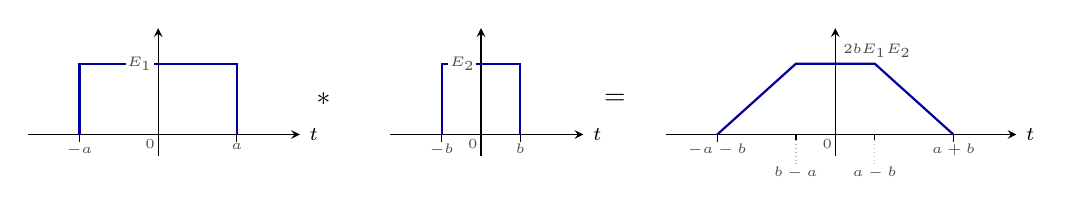
\begin{tikzpicture}[x=0.5cm,y=0.9cm]
  \begin{scope}
    \taxes{-3.3}{3.6}{1.5}{-0.3}
    \rectp{-2}{2}{1}
    \xt{-2}{-a}\xt{2}{a}\yt{1}{E_1}
  \end{scope}
  \node at (4.2,0.5) {$*$};
  \begin{scope}[xshift=4.1cm]
    \taxes{-2.3}{2.6}{1.5}{-0.3}
    \rectp{-1}{1}{1}
    \xt{-1}{-b}\xt{1}{b}\yt{1}{E_2}
  \end{scope}
  \node at (11.6,0.5) {$=$};
  \begin{scope}[xshift=8.6cm]
    \taxes{-4.3}{4.6}{1.5}{-0.3}
    \draw[sig] (-3,0) -- (-1,1) -- (1,1) -- (3,0);
    \xt{-3}{-a-b}\xt{3}{a+b}
    \xtl{-1}{b-a}{-0.42}\xtl{1}{a-b}{-0.42}
    \node[font=\tiny,gray!60!black,anchor=south west,fill=white,inner sep=0.6pt] at (0.15,1.05) {$2bE_1E_2$};
  \end{scope}
\end{tikzpicture}
\caption{两个不等宽方波（$a>b$）卷积得到梯形：斜边宽 $2b$，顶部宽 $2(a-b)$，顶部高 $2bE_1E_2$。}
\label{fig:trap}
\end{figure}

\example{梯形}{$4\Sa(2\omega)\Sa(\omega)$}{}
$x(t)$ 是转折点为 $-3,-1,1,3$、顶部高 $1$ 的梯形。由 $a+b=3$、$a-b=1$ 解出 $a=2$、$b=1$：它是 $-2\sim2$ 的方波与 $-1\sim1$ 的方波的卷积，前者贡献 $\Sa(2\omega)$，后者贡献 $\Sa(\omega)$。前面的系数仍然是面积，道理与三角波相同（两个 $\Sa$ 在 $0$ 处都等于 $1$）：上底 $2$、下底 $6$、高 $1$，面积 $\frac{(2+6)\times1}2=4$。
\[
X(j\omega)=4\Sa(2\omega)\Sa(\omega).
\]

\subsection{卷积与时移、线性结合}\label{sub:conv-shift}
\example{两个分开的三角波}{$2\Sa^2\big(\tfrac12\omega\big)\cos(3\omega)$}{}
$x(t)$ 由两个三角波组成：一个在 $-4\sim-2$、顶点在 $-3$，一个在 $2\sim4$、顶点在 $3$，高都是 $1$。

\point{分解动作。}
\begin{enumerate}[nosep]
\item $-1\sim1$ 上高 $1$ 的三角波，是两个 $-\frac12\sim\frac12$ 方波的卷积，贡献 $\Sa^2(\frac12\omega)$；面积 $\frac{2\times1}2=1$：
\[
\text{中间的三角波}\xrightarrow{\F}\Sa^2\big(\tfrac12\omega\big).
\]
\item 右移 $3$ 个单位（设中间的为 $x_0(t)$，这里是 $x_0(t-3)$），由时移性质乘 $e^{-j3\omega}$：$\Sa^2(\frac12\omega)e^{-j3\omega}$。
\item 左移 $3$ 个单位（$x_0(t+3)$），乘 $e^{j3\omega}$：$\Sa^2(\frac12\omega)e^{j3\omega}$。
\item 由线性性质相加：
\[
X(j\omega)=\Sa^2\big(\tfrac12\omega\big)\big[e^{-j3\omega}+e^{j3\omega}\big]=2\Sa^2\big(\tfrac12\omega\big)\cos(3\omega).
\]
\end{enumerate}
\point{连续动作。}这正是「关于纵轴对称复制」：中间的三角波写出 $\Sa^2(\frac12\omega)$，乘 $2\cos(3\omega)$。这些推理练熟以后，都能一步写出。

\example{斜坡接常数}{$\dfrac1{j\omega}\Sa\big(\tfrac12\omega\big)e^{j\frac12\omega}+\pi\delta(\omega)$}{}
$x(t)$ 在 $t<-1$ 时为 $0$，在 $-1\sim0$ 上从 $0$ 线性升到 $1$，$t>0$ 后一直为 $1$（图~\ref{fig:ramp}）。这是目前用卷积求变换的题里较难的一道（除了符号函数之外）。

\point{关键：看出它是一个卷积。}
\[
x(t)=\big[\,-1\sim0\text{ 上高 }1\text{ 的方波}\,\big]*u(t).
\]
方波与 $u(t)$ 卷积，就是对方波从 $-\infty$ 积分到 $t$：在 $-1\sim0$ 上积分值线性增加到 $1$，之后保持 $1$。

方波的半宽是 $\frac12$、面积是 $1$，它是 $-\frac12\sim\frac12$ 的方波左移 $\frac12$，所以变换是 $\Sa(\frac12\omega)e^{j\frac12\omega}$。时域卷积等于频域相乘：
\[
\begin{aligned}
X(j\omega)&=\Sa\big(\tfrac12\omega\big)e^{j\frac12\omega}\Big[\frac1{j\omega}+\pi\delta(\omega)\Big]\\
&=\frac1{j\omega}\Sa\big(\tfrac12\omega\big)e^{j\frac12\omega}+\pi\delta(\omega).
\end{aligned}
\]
化简第二项用了 $x(\omega)\delta(\omega)=x(0)\delta(\omega)$：$\omega=0$ 时 $\Sa(0)=1$、$e^{j0}=1$。

\point{其他做法。}
\begin{itemize}[nosep]
\item 硬算：拆成 $-1\sim1$ 上的一段加 $u(t)$，斜坡那段硬积分，再相加。只要算对，结果一样。
\item 拆成无穷多个三角波：$-1\sim1$ 上高 $1$ 的三角波，加上它右移 $1$、右移 $2$、……，一直加下去，正好是 $x(t)$。于是
\[
X(j\omega)=\Sa^2\big(\tfrac12\omega\big)\big[1+e^{-j\omega}+e^{-j2\omega}+\cdots\big],
\]
再对括号里的无穷级数求和。思路是对的，但不是最简单的，级数求和也不好化。
\end{itemize}

\begin{figure}[H]
\centering
\begin{tikzpicture}[x=0.6cm,y=0.9cm]
  \begin{scope}
    \taxes{-2.3}{3.6}{1.5}{-0.3}
    \draw[sig] (-2.2,0) -- (-1,0) -- (0,1) -- (3.4,1);
    \xt{-1}{-1}\ytr{1}{1}
    \node[font=\footnotesize,anchor=south] at (0,1.5) {$x(t)$};
  \end{scope}
  \node at (4.5,0.5) {$=$};
  \begin{scope}[xshift=4.6cm]
    \taxes{-2.3}{1.6}{1.5}{-0.3}
    \rectp{-1}{0}{1}
    \xt{-1}{-1}\ytr{1}{1}
  \end{scope}
  \node at (10.0,0.5) {$*$};
  \begin{scope}[xshift=7.4cm]
    \taxes{-1.3}{3.6}{1.5}{-0.3}
    \draw[sig] (-1.2,0) -- (0,0) -- (0,1) -- (3.4,1);
    \yt{1}{1}
    \node[font=\footnotesize,anchor=south] at (0,1.5) {$u(t)$};
  \end{scope}
\end{tikzpicture}
\caption{斜坡接常数的信号，等于 $-1\sim0$ 上的方波与 $u(t)$ 的卷积，即方波的累积积分。}
\label{fig:ramp}
\end{figure}

%==================================================================
\section{综合练习}\label{sec:drill}
下面四题都不是那么直观，但都可以用前面的积木和规则做出来。

\begin{figure}[H]
\centering
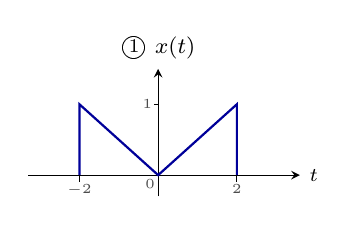
\begin{tikzpicture}[x=0.5cm,y=0.9cm]
  \taxes{-3.3}{3.6}{1.5}{-0.3}
  \draw[sig] (-2,0) -- (-2,1) -- (0,0) -- (2,1) -- (2,0);
  \xt{-2}{-2}\xt{2}{2}\yt{1}{1}
  \node[font=\footnotesize,anchor=south] at (0,1.5) {\cn1\ $x(t)$};
\end{tikzpicture}
\hspace{4mm}
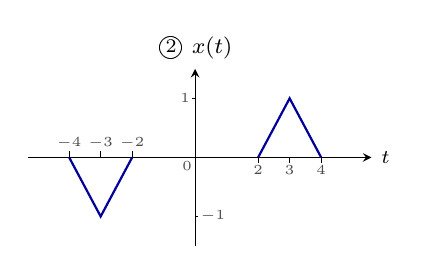
\begin{tikzpicture}[x=0.4cm,y=0.75cm]
  \taxes{-5.3}{5.6}{1.5}{-1.5}
  \trip{2}{3}{4}{1}\trip{-4}{-3}{-2}{-1}
  \xt{2}{2}\xt{3}{3}\xt{4}{4}\xtu{-4}{-4}\xtu{-3}{-3}\xtu{-2}{-2}
  \yt{1}{1}\ytr{-1}{-1}
  \node[font=\footnotesize,anchor=south] at (0,1.5) {\cn2\ $x(t)$};
\end{tikzpicture}
\hspace{4mm}
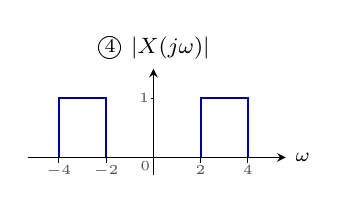
\begin{tikzpicture}[x=0.3cm,y=0.75cm]
  \taxes[\omega]{-5.3}{5.6}{1.5}{-0.3}
  \rectp{-4}{-2}{1}\rectp{2}{4}{1}
  \xt{-4}{-4}\xt{-2}{-2}\xt{2}{2}\xt{4}{4}\yt{1}{1}
  \node[font=\footnotesize,anchor=south] at (0,1.5) {\cn4\ $|X(j\omega)|$};
\end{tikzpicture}
\hspace{2mm}
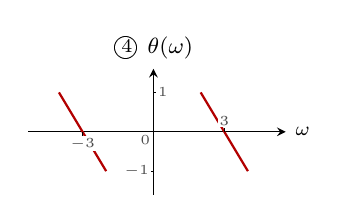
\begin{tikzpicture}[x=0.3cm,y=0.5cm]
  \taxes[\omega]{-5.3}{5.6}{1.6}{-1.6}
  \draw[res] (-4,1) -- (-2,-1); \draw[res] (2,1) -- (4,-1);
  \xtu{3}{3}\xt{-3}{-3}\ytr{1}{1}\yt{-1}{-1}
  \node[font=\footnotesize,anchor=south] at (0,1.6) {\cn4\ $\theta(\omega)$};
\end{tikzpicture}
\caption{综合练习的已知条件。\cn1 V 形信号；\cn2 一正一负两个三角波；\cn4 幅度谱是 $\pm3$ 附近宽 $2$ 的两个方波，相位在每一段上是斜率 $-1$（$45^\circ$ 向下）的直线，在 $\pm3$ 处为 $0$。\cn3 给的是频域表达式，没有画图。}
\label{fig:drill}
\end{figure}

\example{V 形信号}{$4\Sa(2\omega)-2\Sa^2(\omega)$}{练习一}
$x(t)$ 在 $-2\sim2$ 上，$t=0$ 处为 $0$，向两边线性升到 $1$（图~\ref{fig:drill}\,\cn1）。它等于 $-2\sim2$ 上高 $1$ 的方波，减掉 $-2\sim2$ 上顶点高 $1$ 的三角波：
\begin{itemize}[nosep]
\item 方波：$\Sa(2\omega)$，面积 $4$，得 $4\Sa(2\omega)$；
\item 三角波：两个 $-1\sim1$ 方波的卷积，写 $\Sa^2(\omega)$；面积 $\frac{4\times1}2=2$，得 $2\Sa^2(\omega)$。
\end{itemize}
\[
X(j\omega)=4\Sa(2\omega)-2\Sa^2(\omega).
\]
\point{易错点。}三角波的系数是面积 $\frac{4\times1}{2}=2$，不是 $4$。

\example{一正一负两个三角波}{$-2j\Sa^2\big(\tfrac12\omega\big)\sin(3\omega)$}{练习二}
右边的三角波在 $2\sim4$、顶点 $(3,1)$；左边的在 $-4\sim-2$、顶点 $(-3,-1)$，朝下（图~\ref{fig:drill}\,\cn2）。
\begin{enumerate}[nosep]
\item $-1\sim1$ 上高 $1$ 的三角波，是两个 $-\frac12\sim\frac12$ 方波的卷积：$\Sa^2(\frac12\omega)$，面积 $\frac{2\times1}{2}=1$；
\item 右移 $3$：$\Sa^2(\frac12\omega)e^{-j3\omega}$；
\item 左移 $3$：$\Sa^2(\frac12\omega)e^{j3\omega}$；
\item 右边的减去左边的（左边朝下），由线性性质：
\[
X(j\omega)=\Sa^2\big(\tfrac12\omega\big)\big[e^{-j3\omega}-e^{j3\omega}\big].
\]
\end{enumerate}
再化简：$e^{j\alpha}-e^{-j\alpha}=2j\sin\alpha$，这里是负指数减正指数，正好反过来，得 $-2j\sin(3\omega)$。所以
\[
X(j\omega)=-2j\Sa^2\big(\tfrac12\omega\big)\sin(3\omega).
\]

\example{频域乘积的反变换}{$-6\sim6$ 上顶点高 $3$ 的三角波}{练习三}
已知 $X(j\omega)=\dfrac{2\sin^2(3\omega)}{\omega^2}$，求 $x(t)$。

\point{拆成两个因式。}
\[
X(j\omega)=\Big[\frac{2\sin(3\omega)}{\omega}\Big]\Big[\frac{\sin(3\omega)}{\omega}\Big].
\]
频域相乘，时域就是卷积。分别求两个因式的反变换：
\begin{itemize}[nosep]
\item $\frac{2\sin(3\omega)}{\omega}=6\Sa(3\omega)$，对应 $-3\sim3$ 上的方波。高度用 $x(0)=\frac1{2\pi}\int X(j\omega)\,\dd\omega$ 定：
\[
\int_{-\infty}^{+\infty}\frac{2\sin(3\omega)}{\omega}\,\dd\omega=2\pi ,
\]
除以 $2\pi$ 得高 $1$。
\item $\frac{\sin(3\omega)}{\omega}$ 对应同样宽度的方波，积分是上面的一半 $\pi$，除以 $2\pi$ 得高 $\frac12$。
\end{itemize}
\point{卷积。}两个长度一致的方波卷积得到三角波，底在 $-6\sim6$；顶点是两个方波完全重合时的值，等于「重叠长度 $6$ $\times1\times\frac12$」：
\[
x(t)=-6\sim6\text{ 上、顶点高 }3\text{ 的三角波}.
\]
验算：三角形面积 $\frac{12\times3}2=18$，而 $X(j0)=\lim_{\omega\to0}\frac{2\sin^2(3\omega)}{\omega^2}=18$，一致。

\example{频域搬移后的反变换}{$x(t)=\dfrac{\sin(t-1)}{\pi(t-1)}\cdot2\cos(3t)$}{练习四}
已知 $|X(j\omega)|$ 是 $-4\sim-2$ 和 $2\sim4$ 上高 $1$ 的两个方波，相位 $\theta(\omega)$ 在每一段上是斜率 $-1$ 的直线，在 $\pm3$ 处为 $0$（图~\ref{fig:drill}\,\cn4）。目前来说这是推起来最不顺手、也最难的一道。

\point{先做一道简单的。}若 $|X(j\omega)|$ 是 $-1\sim1$ 上高 $1$ 的方波，$\theta(\omega)=-\omega$（$45^\circ$ 向下的直线）。只有幅度时，由公式 \cn5（$\omega_c=1$）对应 $\frac{\sin t}{\pi t}$；乘上 $e^{j\theta(\omega)}=e^{-j\omega}$，线性相位对应延时 $1$，所有的 $t$ 换成 $t-1$：
\[
\frac{\sin(t-1)}{\pi(t-1)}\xrightarrow{\F}|X(j\omega)|\text{ 为 }-1\sim1\text{ 的方波},\ \theta(\omega)=-\omega .
\]
\point{频域右移 $3$。}由频移性质（教材第 104 页式 3-43），$x(t)e^{j\omega_0t}\xrightarrow{\F}X(j(\omega-\omega_0))$，取 $\omega_0=3$：
\[
\frac{\sin(t-1)}{\pi(t-1)}\,e^{j3t}\xrightarrow{\F}\text{上面的频谱整体右移 }3\text{：幅度在 }2\sim4\text{，相位 }-(\omega-3).
\]
\point{频域左移 $3$。}同理
\[
\frac{\sin(t-1)}{\pi(t-1)}\,e^{-j3t}\xrightarrow{\F}\text{整体左移 }3\text{：幅度在 }-4\sim-2\text{，相位 }-(\omega+3).
\]
\point{相加。}两段频谱加起来正好是题目给的 $X(j\omega)$，时域两项相加，$e^{j3t}+e^{-j3t}=2\cos(3t)$：
\[
x(t)=\frac{\sin(t-1)}{\pi(t-1)}\cdot2\cos(3t).
\]
\point{连续动作。}与时域的「对称复制」对应：\textbf{频域里同一个东西沿纵轴左右对称地复制，时域就乘以 $2\cos(\omega_0t)$}。知道这一点可以一步写出答案。

%==================================================================
\section{用卷积性质重新考查 LTI 系统}\label{sec:lti}
卷积性质不只是用来做题。通过它，对线性时不变(LTI)系统的整个性质会有更深刻的理解。

\begin{figure}[H]
\centering
\begin{tikzpicture}
  \node (x) at (0,0) {$x(t)$};
  \node[blk] (h) at (2.4,0) {$h(t)$};
  \node[anchor=west] (y) at (4.4,0) {$y(t)=x(t)*h(t)$};
  \draw[->] (x) -- (h); \draw[->] (h) -- (y);
  \node[anchor=west,font=\footnotesize,gray!60!black] at (9.4,0) {时域};
  \node (X) at (0,-1.3) {$X(j\omega)$};
  \node[blk] (H) at (2.4,-1.3) {$H(j\omega)$};
  \node[anchor=west] (Y) at (4.4,-1.3) {$Y(j\omega)=X(j\omega)H(j\omega)$};
  \draw[->] (X) -- (H); \draw[->] (H) -- (Y);
  \node[anchor=west,font=\footnotesize,gray!60!black] at (9.4,-1.3) {频域};
  \draw[->,gray] (0,-0.3) -- node[left,font=\scriptsize] {$\F$} (0,-1.0);
  \draw[->,gray] (2.4,-0.4) -- node[left,font=\scriptsize] {$\F$} (2.4,-0.9);
\end{tikzpicture}
\caption{LTI 系统的时域画法与频域画法。由时域卷积性质，两张图表达的意思完全一样。}
\label{fig:lti}
\end{figure}

时域里，输出等于输入卷积冲激响应；对所有信号做傅里叶变换以后，输出的频谱等于输入的频谱乘以冲激响应的频谱。频域的图里有时不写「LTI」，只要是这样的图，讨论的就是线性时不变系统。由 $Y(j\omega)=X(j\omega)H(j\omega)$，
\begin{remember}
\[
H(j\omega)=\frac{Y(j\omega)}{X(j\omega)} .
\]
$H(j\omega)$ 是冲激响应 $h(t)$ 的傅里叶变换，也叫 LTI 系统的\textbf{系统函数}(system function)。有的书把时域的 $h(t)$ 也叫系统函数，两种叫法都有道理。

学完第三章的最高境界，是看 $h(t)$ 和看 $H(j\omega)$ 在眼里是同一个东西：看时域和看频域，看到的是同一个东西。
\end{remember}

\subsection{已知输入和输出，求冲激响应}\label{sub:findh}
第三章开头（第 09 篇）留下的问题：$x(t)$ 是 $0\sim2$ 上高 $1$ 的方波，卷积未知的 $h(t)$，得到 $y(t)$ 是 $0\sim2$ 上、顶点 $(1,1)$ 的三角波。求 $h(t)$。现在一步一步推出 MATLAB 作业里的那个公式。

\begin{figure}[H]
\centering
\begin{tikzpicture}[x=0.65cm,y=0.9cm]
  \begin{scope}
    \taxes{-1.3}{3.4}{1.5}{-0.3}
    \rectp{0}{2}{1}
    \xt{2}{2}\yt{1}{1}
    \node[font=\footnotesize,anchor=south] at (0,1.5) {$x(t)$};
  \end{scope}
  \node at (4.9,0.5) {$*\ h(t)\ =$};
  \begin{scope}[xshift=5.6cm]
    \taxes{-1.3}{3.4}{1.5}{-0.3}
    \trip{0}{1}{2}{1}
    \xt{1}{1}\xt{2}{2}\yt{1}{1}
    \node[font=\footnotesize,anchor=south] at (0,1.5) {$y(t)$};
  \end{scope}
\end{tikzpicture}
\caption{已知方波输入与三角波输出，求冲激响应 $h(t)$。}
\label{fig:findh}
\end{figure}

\point{第一步：输入的变换。}$x(t)$ 是 $-1\sim1$ 的方波右移 $1$：$\Sa(\omega)$，面积 $2$，再乘 $e^{-j\omega}$：
\[
X(j\omega)=2\Sa(\omega)\,e^{-j\omega}.
\]
\point{第二步：输出的变换。}$y(t)$ 是 $-1\sim1$、顶点高 $1$ 的三角波右移 $1$。三角波由两个 $-\frac12\sim\frac12$ 的方波卷积而成，写 $\Sa^2(\frac12\omega)$；面积 $\frac{2\times1}{2}=1$；再乘 $e^{-j\omega}$：
\[
Y(j\omega)=\Sa^2\big(\tfrac12\omega\big)\,e^{-j\omega}.
\]
这些变换现在写得比较快，其实中间隐含了前面那些分解动作；不清楚的话，回头把每一步补出来。

\point{第三步：相除。}两个 $e^{-j\omega}$ 消掉：
\[
H(j\omega)=\frac{Y(j\omega)}{X(j\omega)}=\frac{\Sa^2(\frac12\omega)}{2\Sa(\omega)}
=\frac{\dfrac{\sin^2(\frac12\omega)}{\frac14\omega^2}}{\dfrac{2\sin\omega}{\omega}}
=\frac{4\sin^2(\frac12\omega)}{\omega^2}\cdot\frac{\omega}{2\sin\omega}
=\frac{2\sin^2(\frac12\omega)}{\omega\sin\omega}.
\]
（$(\frac12\omega)^2=\frac14\omega^2$，$\frac14$ 拿到分子变成 $4$；分子分母的 $\omega$ 约掉一个，$4$ 与 $2$ 约成 $2$。）

\point{第四步：反变换。}
\[
h(t)=\frac1{2\pi}\int_{-\infty}^{+\infty}H(j\omega)\,e^{j\omega t}\,\dd\omega
=\frac1{2\pi}\int_{-\infty}^{+\infty}\frac{2\sin^2(\frac12\omega)}{\omega\sin\omega}\big[\cos(\omega t)+j\sin(\omega t)\big]\dd\omega .
\]
分析奇偶性：分子 $\sin(\frac12\omega)$ 是奇函数，平方后是偶函数；分母 $\omega$ 和 $\sin\omega$ 都是奇函数，相乘是偶函数；偶函数除以偶函数，$H(j\omega)$ 是 $\omega$ 的偶函数。它乘奇函数 $\sin(\omega t)$ 得奇函数，在对称区间上积分为 $0$。只剩余弦一项：
\[
h(t)=\frac1{2\pi}\int_{-\infty}^{+\infty}\frac{2\sin^2(\frac12\omega)}{\omega\sin\omega}\cos(\omega t)\,\dd\omega .
\]
这就是第 09 篇 MATLAB 作业里给出的公式（与那里的 $\frac1\pi\int\frac{\sin^2(\omega/2)}{\omega\sin\omega}\cos(\omega t)\,\dd\omega$ 相同）。

\begin{remember}
\textbf{已知 $x(t)$、$y(t)$ 求 $h(t)$ 的步骤：}把 $x(t)$ 和 $y(t)$ 分别做傅里叶变换；两者相除得到 $H(j\omega)$；再用反变换公式得到时域的 $h(t)$。这就回答了第三章开头的问题。
\end{remember}
被积函数在 $\omega=\pi,3\pi,5\pi,\dots$ 处趋于无穷大，这个积分不是普通意义下收敛的积分，所以数值算出的 $h(t)$ 振荡剧烈；从时域直接求出的 $h(t)$ 见第 09 篇最后一节。

\subsection{一对输入输出确定整个 LTI 系统}\label{sub:onepair}
\point{判断题。}对于线性时不变系统，如果知道了它的\textbf{任何一个不为零的输入}对应的输出，就知道了它对所有输入的输出。这句话对吗？

\point{答：对。}这里限制得很死，「不为零」三个字不能少。

\begin{itemize}[nosep]
\item 如果去掉「不为零」，这句话就错了：输入为零时，LTI 系统的输出一定为零（由线性很容易推出），这一对输入输出不提供任何信息。
\item 输入不为零，$x(t)$ 不为零，$X(j\omega)$ 也不为零。知道 $x(t)$ 经过系统得到 $y(t)$，就知道 $X(j\omega)$ 经过系统得到 $Y(j\omega)$，直接算出系统函数 $H(j\omega)=\frac{Y(j\omega)}{X(j\omega)}$，再做反变换得到 $h(t)$。
\item 另外任何一个输入 $x_1(t)$，输出都是 $x_1(t)*h(t)$。
\end{itemize}

\begin{remember}
LTI 系统是一个非常简单的系统：它的全部性质被\textbf{任何一对不为零的输入和输出}完全确定。
\end{remember}

\begin{note}
上面的论证要用 $\frac{Y(j\omega)}{X(j\omega)}$，严格地说需要 $X(j\omega)$ 在各个频率上都不为零（个别孤立的零点不影响积分）。如果 $X(j\omega)$ 在一整段频率上为零，那一段上的 $H(j\omega)$ 就定不出来。例如输入 $x(t)=\frac{\sin t}{\pi t}$，它的频谱只在 $-1\sim1$ 上不为零：恒等系统 $H(j\omega)=1$ 和 $-2\sim2$ 上为 $1$ 的理想低通 $H(j\omega)$，对这个输入的输出都是 $\frac{\sin t}{\pi t}$，但两个系统不同。所以「不为零的输入」应理解为频谱不在一整段频率上为零的输入。
\end{note}

%==================================================================
\section{积分性质}\label{sec:int}
\begin{remember}
\textbf{积分性质（教材 3.4.5，第 107 页最上面的公式）。}若 $x(t)\xrightarrow{\F}X(j\omega)$，则
\[
\int_{-\infty}^{t}x(\tau)\,\dd\tau\xrightarrow{\F}\frac{X(j\omega)}{j\omega}+\pi X(j0)\,\delta(\omega).
\]
\end{remember}
这个公式不需要记，它可以由卷积性质顺理成章地得到。

\point{推导。}第二章的补充知识讲过，
\[
\int_{-\infty}^{t}x(\tau)\,\dd\tau=x(t)*u(t).
\]
时域卷积等于频域相乘，$u(t)\xrightarrow{\F}\frac1{j\omega}+\pi\delta(\omega)$：
\[
\F\Big[\int_{-\infty}^{t}x(\tau)\,\dd\tau\Big]=X(j\omega)\Big[\frac1{j\omega}+\pi\delta(\omega)\Big]
=\frac{X(j\omega)}{j\omega}+\pi X(j\omega)\delta(\omega).
\]
再用 $X(j\omega)\delta(\omega)=X(j0)\delta(\omega)$，$\omega$ 换成 $0$，就得到上面的公式。

\begin{figure}[H]
\centering
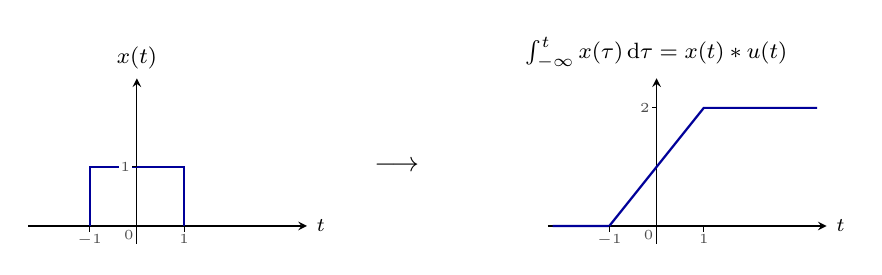
\begin{tikzpicture}[x=0.6cm,y=0.75cm]
  \begin{scope}
    \taxes{-2.3}{3.6}{2.5}{-0.3}
    \rectp{-1}{1}{1}
    \xt{-1}{-1}\xt{1}{1}\yt{1}{1}
    \node[font=\footnotesize,anchor=south] at (0,2.5) {$x(t)$};
  \end{scope}
  \node at (5.5,1) {$\longrightarrow$};
  \begin{scope}[xshift=6.6cm]
    \taxes{-2.3}{3.6}{2.5}{-0.3}
    \draw[sig] (-2.2,0) -- (-1,0) -- (1,2) -- (3.4,2);
    \xt{-1}{-1}\xt{1}{1}\yt{2}{2}
    \node[font=\footnotesize,anchor=south] at (0,2.5) {$\int_{-\infty}^{t}x(\tau)\,\dd\tau=x(t)*u(t)$};
  \end{scope}
\end{tikzpicture}
\caption{$-1\sim1$ 上高 $1$ 的方波，累积积分在 $-1\sim1$ 上线性升到面积 $2$，之后保持不变。最终值 $2=X(j0)$，它决定了积分性质里冲激项的强度 $\pi X(j0)$。}
\label{fig:int}
\end{figure}

%==================================================================
\section{连续时间 LTI 系统的频域分析}\label{sec:freqana}
教材 3.5 节（第 116 页）。下面三道例题都很简单，但要通过它们建立几个概念。

\point{概念。}求一个 LTI 系统的 $h(t)$，就是把输入换成 $\delta(t)$ 送进系统，得到的输出就是 $h(t)$（冲激响应，也叫系统函数）；$h(t)$ 知道了，它的傅里叶变换 $H(j\omega)$ 自然也就知道了。这个定义心里一定要清楚。

\example{微分器}{$H(j\omega)=j\omega$}{教材例 3-11}
微分器 $y(t)=\frac{\dd x(t)}{\dd t}$，把输入求导，是第一章的内容；第一章也严格证明过微分器是 LTI 系统。把 $x(t)$ 换成 $\delta(t)$：
\[
h(t)=\frac{\dd\delta(t)}{\dd t}=\delta'(t).
\]
由时域微分性质 $\frac{\dd x(t)}{\dd t}\xrightarrow{\F}j\omega X(j\omega)$，以及 $\delta(t)\xrightarrow{\F}1$，得 $\delta'(t)\xrightarrow{\F}j\omega\cdot1$：
\[
H(j\omega)=j\omega .
\]

\example{积分器}{$H(j\omega)=\dfrac1{j\omega}+\pi\delta(\omega)$}{教材例 3-12}
积分器 $y(t)=\int_{-\infty}^{t}x(\tau)\,\dd\tau$，也是第一章讲过的。把 $x$ 换成 $\delta$：
\[
h(t)=\int_{-\infty}^{t}\delta(\tau)\,\dd\tau=\begin{cases}1,& t>0\\0,& t<0\end{cases}=u(t).
\]
$t>0$ 时积分区间覆盖了 $\delta(\tau)$ 有值的那个点，积出来是 $1$；$t<0$ 时没有积到那个点，积出来是 $0$。于是
\[
H(j\omega)=\F[u(t)]=\frac1{j\omega}+\pi\delta(\omega).
\]
\point{另一种方式。}$y(t)=\int_{-\infty}^{t}x(\tau)\,\dd\tau=x(t)*u(t)$，又 $y(t)=x(t)*h(t)$，直接看出 $h(t)=u(t)$。两种方式得到的 $h(t)$ 必须一样，否则整个 LTI 系统的理论就矛盾了。

\example{延时器}{$h(t)=\delta(t-t_0)$，$H(j\omega)=e^{-j\omega t_0}$}{教材例 3-13}
延时器 $y(t)=x(t-t_0)$。$h(t)$ 是输入为 $\delta(t)$ 时的输出，直接把 $x$ 换成 $\delta$：
\[
h(t)=\delta(t-t_0).
\]
\point{分解动作。}由时移性质 $x(t-t_0)\xrightarrow{\F}X(j\omega)e^{-j\omega t_0}$，$\delta(t)\xrightarrow{\F}1$，所以 $\delta(t-t_0)\xrightarrow{\F}e^{-j\omega t_0}$：
\[
H(j\omega)=e^{-j\omega t_0}.
\]
\point{另一种方式。}对 $y(t)=x(t-t_0)$ 两边直接做傅里叶变换：$Y(j\omega)=X(j\omega)e^{-j\omega t_0}$，对照 $Y(j\omega)=X(j\omega)H(j\omega)$，直接得到 $H(j\omega)=e^{-j\omega t_0}$。两种方式没有矛盾。

\begin{figure}[H]
\centering
\begin{tikzpicture}[x=0.5cm,y=0.55cm]
  \taxes[\omega]{-3.3}{3.6}{3.4}{-0.3}
  \draw[res] (-3,3) -- (0,0) -- (3,3);
  \xt{-2}{-2}\xt{2}{2}\yt{2}{2}
  \node[font=\footnotesize,anchor=south] at (0,3.4) {微分器 $|H(j\omega)|=|\omega|$};
\end{tikzpicture}
\hspace{5mm}
\begin{tikzpicture}[x=0.5cm,y=0.55cm]
  \taxes[\omega]{-3.3}{3.6}{3.4}{-0.3}
  \draw[res,domain=0.34:3.2,samples=60] plot (\x,{1/\x});
  \draw[res,domain=-3.2:-0.34,samples=60] plot (\x,{-1/\x});
  \draw[imp,sig] (0,0) -- (0,2.4);
  \node[font=\scriptsize,anchor=west,sig] at (0.1,2.4) {$(\pi)$};
  \xt{-1}{-1}\xt{1}{1}\ytr{1}{1}
  \node[font=\footnotesize,anchor=south] at (0,3.4) {积分器 $\frac1{|\omega|}$ 与 $\pi\delta(\omega)$};
\end{tikzpicture}
\hspace{5mm}
\begin{tikzpicture}[x=0.5cm,y=0.55cm]
  \taxes[\omega]{-3.3}{3.6}{3.4}{-3.4}
  \draw[sig] (-3.2,1) -- (3.2,1);
  \draw[res] (-3,3) -- (3,-3);
  \xt{2}{2}\xtu{-2}{-2}\yt{1}{1}
  \node[font=\footnotesize,anchor=south] at (0,3.4) {延时器};
  \node[sig,font=\scriptsize,anchor=south west] at (1.4,1) {$|H|=1$};
  \node[res,font=\scriptsize,anchor=west] at (-3.2,-1.6) {$\theta=-\omega t_0$};
\end{tikzpicture}
\caption{三个系统的频率响应。微分器放大高频；积分器放大低频，$\omega=0$ 处还有冲激；延时器幅度处处为 $1$，只引入线性相位（图中取 $t_0=1$）。}
\label{fig:systems}
\end{figure}

\end{document}
